\documentclass[sigplan]{acmart}\settopmatter{printfolios=true,printccs=false,printacmref=false}
\usepackage{flushend}

% What is the type of a cell in Python? Only the result? You say exports must 
% be explicitly defined - so the type of the cell is the type of the export?

% The authors say (page 2), "The data store keeps version
% history and annotates data with metdata such as types, inferred
% semantics and provenance information."  How these semantics and
% provenance information are inferred and represented, however, is
% not elaborated on (but only very briefly mentioned in Section 3.3,
% bottom of page 3).  The role of provenance thus remains unclear to me.

% How does Wrattler compare to other notebook systems in terms of storage and compute overhead, 
% since a) extra data needs to be maintained, and 
%  b) the state and the runtime are now separated? It would be great to include some (preliminary) numbers in this regard. 



\acmConference[TaPP 2018]{10th USENIX Workshop on The Theory and Practice of Provenance}{July 11--12, 2018}{London, UK}
\acmYear{2018}
\acmISBN{} % \acmISBN{978-x-xxxx-xxxx-x/YY/MM}
\acmDOI{} % \acmDOI{10.1145/nnnnnnn.nnnnnnn}
\startPage{1}
\setcopyright{rightsretained}

\bibliographystyle{ACM-Reference-Format}

\begin{document}
\title{Wrattler: \textnormal{Reproducible, live and polyglot notebooks}}

\author{Tomas Petricek}
\affiliation{
  \institution{University of Kent}
}
\affiliation{
  \institution{The Alan Turing Institute}
}
\email{tomas@tomasp.net}
\author{James Geddes}
\affiliation{
  \institution{The Alan Turing Institute}
}
\email{jgeddes@turing.ac.uk}
\author{Charles Sutton}
\affiliation{
  \institution{The University of Edinburgh}
}
\affiliation{
  \institution{The Alan Turing Institute and Google}
}
\email{csutton@inf.ed.ac.uk}

\definecolor{cmtclr}{rgb}{0.0,0.6,0.0}
\definecolor{kvdclr}{rgb}{0.0,0.0,0.6}
\definecolor{numclr}{rgb}{0.0,0.4,0.0}
\definecolor{strclr}{rgb}{0.4,0.4,0.0}
\definecolor{rstrclr}{rgb}{0.5,0.1,0.0}
\definecolor{prepclr}{rgb}{0.6,0.0,0.2}
\newcommand{\vect}[1]{\langl #1 \rangl}
\newcommand{\langl}{\begin{picture}(4.5,7)
\put(1.1,2.5){\rotatebox{60}{\line(1,0){5.5}}}
\put(1.1,2.5){\rotatebox{300}{\line(1,0){5.5}}}
\end{picture}}
\newcommand{\rangl}{\begin{picture}(4.5,7)
\put(.9,2.5){\rotatebox{120}{\line(1,0){5.5}}}
\put(.9,2.5){\rotatebox{240}{\line(1,0){5.5}}}
\end{picture}}
\newcommand{\ball}[1]{\FPeval{\result}{clip(201+#1)}\textnormal{\ding{\result}}}
\newcommand{\lsep}{~\,|\,~}
\newcommand{\num}[1]{\textcolor{numclr}{#1}}
\newcommand{\str}[1]{\textnormal{\textcolor{strclr}{\sffamily "#1"}}}
\newcommand{\strf}[1]{\textnormal{\textcolor{strclr}{\sffamily #1}}}
\newcommand{\rstr}[1]{\textnormal{\textcolor{rstrclr}{\sffamily "#1"}}}
\newcommand{\ident}[1]{\textnormal{\sffamily #1}}
\newcommand{\qident}[1]{\textnormal{\sffamily \textquotesingle #1\textquotesingle}}
\newcommand{\dom}{\ident{dom}}
\newcommand{\kvd}[1]{\textnormal{\textcolor{kvdclr}{\sffamily #1}}}

\newcommand{\bndclr}[1]{\textcolor{kvdclr}{#1}}
\newcommand{\bkndclr}[1]{\textcolor{prepclr}{#1}}
\newcommand{\blblclr}[1]{\textcolor{numclr}{#1}}
\newcommand{\bnd}[1]{\textnormal{\textcolor{kvdclr}{\sffamily #1}}}
\newcommand{\bknd}[1]{\textnormal{\textcolor{prepclr}{\sffamily #1}}}
\newcommand{\blbl}[1]{\textnormal{\textcolor{numclr}{\sffamily #1}}}

\begin{abstract}
Notebooks such as Jupyter became a popular environment for data science, because 
they support interactive data exploration and provide a convenient way of interleaving code, 
comments and visualizations. Alas, most notebook systems use an architecture that leads to a 
limited model of interaction and makes reproducibility and versioning difficult.

In this paper, we present Wrattler, a new notebook system built around provenance that addresses
the above issues. Wrattler separates state management from script evaluation and controls the 
evaluation using a dependency graph maintained in the web browser. This allows richer forms of 
interactivity, an efficient evaluation through caching, guarantees reproducibility and makes it 
possible to support versioning.
\end{abstract}
%\keywords{notebook, dependency graph, live coding}
\maketitle

\section{Introduction}
Notebooks \cite{ipython,jupyter} are literate programming \cite{literate} systems
that allow interleaving text, code and outputs. To aid reproducible, 
exploratory data science, notebook systems should provide:

\vspace{-0.3em}
\paragraph{Richer interaction model.}
Web browsers are increasingly powerful and allow moving parts of data exploration to the client-side. 
Notebooks should leverage this and give live previews when writing code to perform simple data exploration.

\vspace{-0.3em}
\paragraph{Transparent state management.}
The state maintained by a notebook should be transparent and accessible to external tools. This
would allow versioning of state and development of tools that provide hints based on the notebook state.

\vspace{-0.3em}
\paragraph{Multiple languages and tools.} 
A notebook should make it easy to combine multiple programming languages. A cell written in one
language should be able to automatically access data frames defined in other languages.

\vspace{-0.3em}
\paragraph{Improved reproducibility.} 
Changing code in a cell should invalidate results that depend on data frames defined in 
the cell. Reverting a change should immediately revert the result to the previous one
and show it immediately using a cache.

\vspace{0.5em}
\noindent
Supporting these is a challenge that combines several research areas. We need programming 
language techniques to efficiently update live previews during editing, provenance methods to 
track data dependencies and data representation that can be shared across langauges.

Wrattler is a new notebook system that supports the above features. We follow a line of work combining 
provenance tracking with notebooks \cite{noworkflow,dataflow}, but rather than extending existing 
systems, we revisit two core aspects of the notebook architecture (Section~\ref{sec:arch}). 
First, Wrattler uses a \emph{dependency graph} to track provenance between cells and even function calls 
inside individual cells (Section~\ref{sec:comp-deps}). When a cell is changed, relevant parts of a graph
are invalidated. This guarantees reproducibility and enables more efficient re-computation.
Second, Wrattler introduces a \emph{data store} that separates state management from code execution 
(Section~\ref{sec:comp-data}). The data store handles versioning and simplifies the support for polyglot programming.

Together, these two changes to the standard architecture of notebook systems make Wrattler notebooks
(Section~\ref{sec:results}) polyglot, reproducible (with an easy and reliable state rollback) and live 
(with efficient re-computation on change that enables live preview during data exploration).

\begin{figure}[b]
\vspace{-2em}
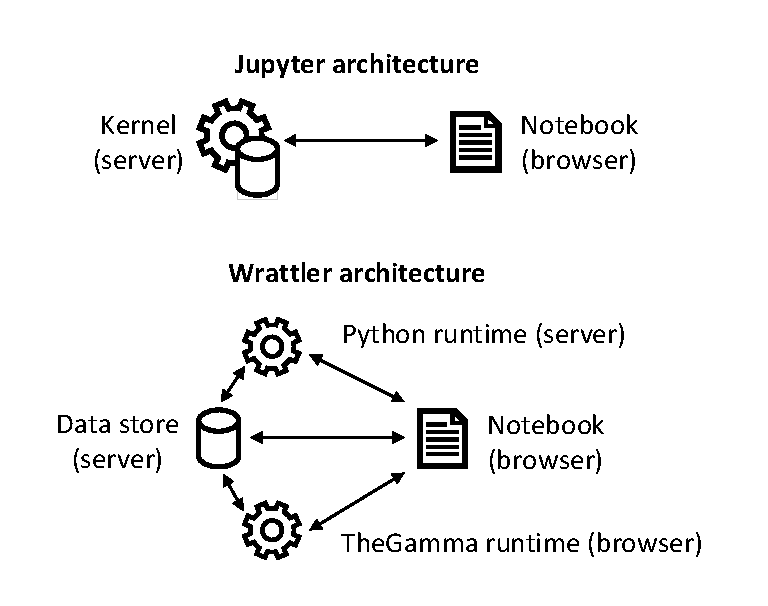
\includegraphics[scale=0.6]{diagram.pdf}
\vspace{-1.5em}
\caption{\small{In notebook systems such as Jupyter, state and execution is managed by a kernel. In
  Wrattler, those functions are split between data store and language runtimes. Language runtimes 
  can run on the server-side (e.g.~Python) or client-side (e.g.~TheGamma).}}
\label{fig:arch}
\end{figure}

\section{Wrattler architecture}
\label{sec:arch}
Standard notebook architecture consists of a \emph{notebook} and a \emph{kernel}. The kernel
runs on a server, evaluates code snippets and maintains state they use.
Notebook runs in a browser and sends commands to the kernel in order to evaluate 
cells selected by the user. As illustrated in Figure~\ref{fig:arch}, Wrattler splits the 
server functionality between two components:

\paragraph{Data store.} Imported external data and results of running scripts  
are stored in the data store. The data store keeps version history and annotates data with 
metadata such as types, inferred semantics and provenance information.

\paragraph{Language runtimes.} Code in notebook cells is evaluated by language runtimes.
The runtimes read input data from and write results back to the data store. Wrattler supports
language runtimes that run code on the server (similar to Jupyter), but also browser-based 
langauge runtimes.

\paragraph{Notebook.} The notebook is displayed in a web browser and orchestrates 
all other components. The browser builds a dependency graph between cells or individual 
calls. It invokes language runtimes to evaluate code that has changed,
and reads data from the data store to display results.  


\begin{figure}
\vspace{-0.5em}
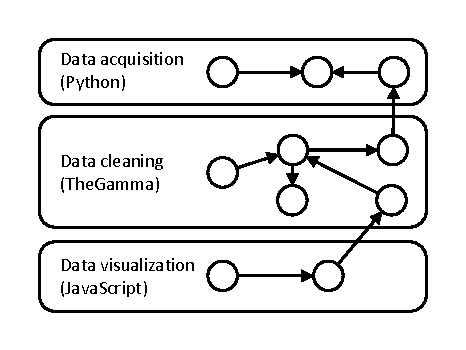
\includegraphics[scale=1,trim=0.5cm 0.5cm 0.5cm 0.5cm]{graph.pdf}
\vspace{-0.5em}
\caption{\small{Dependency graph of a sample notebook: The first (Python) cell downloads data and 
exports the result as a data frame; the second (TheGamma) cell performs data cleaning and the third 
(JavaScript) cell creates a visualization. Language runtime for TheGamma runs in the browser and 
creates a fine-grained graph (which allows an efficient live previews), while Python and JavaScript 
runtimes create just one node for the whole source code.}}
\label{fig:deps}
\vspace{-1em}
\end{figure}

\section{Wrattler components}
\label{sec:comp}

Wrattler runs in the web browser and communicates with the data store and language runtimes
that may run on the server or in the browser. An example of browser-based language runtime is
TheGamma \cite{thegamma}, discussed in Section~\ref{sec:comp-gamma}.

\subsection{Dependency graph}
\label{sec:comp-deps}

At runtime, Wrattler maintains a dependency graph that is composed from sub-graphs
created by individual language runtimes. The graph is acyclic and a node can only depend on earlier 
nodes. Each node has a value which may be:
%
\begin{itemize}
\item A language-specific value that Wrattler does not understand. This is kept in the browser
  and re-computed when the notebook is re-opened.
\item A data frame. Data frame is stored in the data store and browser keeps a reference (URL) 
  of the frame. This is understood by all language runtimes and provides a way of exchanging
  data between multiple languages. 
\end{itemize}
%
Figure~\ref{fig:deps} shows a sample dependency graph. Wrattler creates two nodes for each cell
(representing the cell and its source code) and a node for each data frame exported by a cell 
(e.g.~the rightmost node in the first cell). Nodes in subsequent cells may depend on data frames
exported by earlier cells.

Wrattler treats data frames in a special way. They are stored in data store and each langauge 
runtime is responsible for loading them into a native language representation (e.g. pandas in 
Python and array of records in JavaScript). 

\paragraph{Dependency graph construction.} 
The dependency graph is updated after every code change. Wrattler invokes individual langauge 
runtimes to parse each cell. Language runtimes that run in the browser (e.g.~TheGamma) produce
a fine-grained syntax tree. The result of parsing the whole notebook is then a list of elements
obtained for each cell.

Wrattler then walks over the syntax tree and binds a dependency graph node
to each syntactic element using a process decribed in Figure~\ref{fig:bind}. 
The \emph{antecedents} of a node are the nodes that it depends on. This typically includes 
inputs for an operation or instance on which a member access is performed. 

\paragraph{Checking and evaluation.} 
Nodes in the dependency graph can be annotated with information such as the evaluated value
of the syntactic element that the node represents. An important property of the binding process
(Figure~\ref{fig:bind}) is that, if there is no change in antecedents of a node, binding will 
return the same node as before. As a result, previously evaluated values attached to nodes
in the graph are reused.

Wrattler re-evaluates parts of the dependency graph on demand and the displayed results and 
visualizations always reflect the current source code in the notebook. When the evaluation 
of a cell is requested, Wrattler recursively evaluates all the antecedents of the node and 
then evaluates the value of the node. The evaluation is delegated to a language
runtime associated with the language of the node:
%
\begin{enumerate}
\item For Python nodes, the language runtime sends the source code, together with its 
  dependencies, to a server that retrieves the dependencies and evaluates the code.
\item For TheGamma and JavaScript nodes, the language runtime collects values of the 
  dependencies and runs the operation that the node represents in the browser.
\end{enumerate}

\subsection{Data store}
\label{sec:comp-data}

The data store enables communication between individual Wrattler components and provides a way for 
persistently storing input data. Data frames stored in the data store are associated with the hash 
produced by the binding process outlined in Figure~\ref{fig:bind} and are immutable. When the 
notebook changes, new nodes with new hashes are created and appended to the data store. This means 
that language runtimes can cache them and avoid fetching data from data store each time they need 
to evaluate a code snippet. 

External inputs imported into Wrattler notebooks (such as downloaded web pages) are stored as 
binary blobs. Data frames are stored in JSON format (as an array of records),
but we intend to use a suitable database in the future. During the binding process 
(Section~\ref{sec:comp-deps}), a langauge runtime identifies imported and exported data frames 
for each cell (e.g.~by static analysis of the code). Those are then represented as hashes (keys)
referring to a location in the data store.

The data store also supports a mechanism for annotating data frames with 
semantic information. Columns can be annotated with primitive data types (date, floating-point 
number) and semantic annotation indicating their meaning (address or longitude and latitude). 
Columns, rows and individual cells of the data frame can also be annotated with custom metadata 
such as their data source or accuracy.

\begin{figure}
\vspace{-1em}
\begin{equation*}
\hspace{-3em}\begin{array}{l}
\kvd{procedure}~\ident{bind}(\textit{cache}, \textit{syn})~=\\
\quad \kvd{let}~h = \ident{hash}(\{\ident{kind}(\textit{syn}) \}\cup \ident{antecedents}(\textit{syn}))\\
\quad \kvd{if}~\ident{not}~\ident{contains}(\textit{cache}, h)~\kvd{then}\\
\quad \quad \kvd{let}~n = \emph{fresh node}\\
\quad \quad \ident{value}(n), \ident{hash}(n) \leftarrow \ident{Unevaluated}, h \\
\quad \quad \ident{set}(\textit{cache}, h, n) \\
\quad \ident{lookup}(\textit{cache}, h)\\
\end{array}
\end{equation*}
\vspace{-0.5em}
\caption{\small{When binding a graph node to a syntactic element, Wrattler first computes
  a set of hashes that uniquely represent the node. This includes hash of the kind of the 
  node (e.g. the source code of a Python node or member name in TheGamma) and hashes
  of all antecedents. If a node with a given hash does not exist in cache, a new node
  is created. We set its hash, indicate that its value has not been evaluated and
  add it to the cache.}}
\label{fig:bind}
\vspace{-1em}
\end{figure}

In addition to storing the raw data, the data store also persistently stores the current and
multiple past versions of the dependency graph constructed from the notebook (saved by an 
explicit checkpoint). This makes it possible to analyse the history of a notebook and track how
data is transformed by the computation in a notebook.

\subsection{TheGamma script}
\label{sec:comp-gamma}

The Wrattler architecture supports languages that can be parsed and evaluated in the browser.
To illustrate this, we integrated Wrattler with TheGamma~\cite{thegamma}, a simple browser-based 
language for data exploration.

The Figure~\ref{fig:gamma} shows TheGamma cell in Wrattler during editing. The example uses
broadband speed data published by the UK government \cite{ofcom} and calculates average download
speed in urban and rural areas, respectively. TheGamma supports a rich interactive model in two ways:
%
\begin{itemize}
\item The script is evaluated on-the-fly during editing and a live preview is shown 
  (below the code editor).
\item All code can be written using autocomplete that offers available members (representing
  aggregation operations). Rather than writing code, user repeatedly selects one of the offered 
  members (which are provided by a type provider \cite{providers} running in the browser).
\end{itemize}

For the purpose of this paper, the most important aspect of TheGamma is that scripts can be 
parsed and evaluated in the browser. This allows more interactive style of data exploration
without round-trips to re-evaluate modified code.

\section{Properties of Wrattler}
\label{sec:results}

The Wrattler architecture outlined in Section~\ref{sec:arch} allowed us to develop a prototype 
system with a number of properties that are difficult to obtain with traditional notebooks.

\subsection{Reproducible, live and smart}
The two most important aspects of the Wrattler architecture are that it separates the state from 
the language runtime (using a data store) and that it keeps a dependency graph based on the current
notebook source code (on the client). The provenance information that is available thanks to this
arhcitecture enable a number of properties.

\paragraph{Reproducibility.} The evaluation outputs displayed in Wrattler notebook always reflect
the current source code. When code changes, Wrattler updates the dependency graph and hides 
invalidated visualizations. Because the data store caches earlier results, it is always possible
to go back without re-evaluating the whole notebook.

\paragraph{Refactoring.} The dependency graph allows us to implement notebook refactoring. 
For example, it is possible to extract only code necessary to produce a given visualization.
For code written in TheGamma, this extracts individual operations; for Python or JavaScript,
we can currently extract code at cell-level granularity.

\paragraph{Live previews.} The dependency graph makes it possible to give 
live previews during development. When code changes, only values for new nodes in the graph 
need to be calculated. The fine-grained structure of the dependency graph for TheGamma 
makes it possible to update previews instantly.

\paragraph{Polyglot.} Sharing the state via data store makes it possible to combine multiple
language runtimes, as long as they support sharing data via data frames. In our prototype, this
includes R, JavaScript and TheGamma script, but the extensibility model allows adding further
languages.

\subsection{Wrattler prototype}

A prototype implementation of the Wrattler system is available on GitHub (\url{http://github.com/wrattler}).
The prototype implements language runtimes for TheGamma script (Section~\ref{sec:comp-gamma}), R
and JavaScript. It builds a dependency graph (Section~\ref{sec:comp-deps})
and uses it to evaluate results of cells. 

The data store (Section~\ref{sec:comp-data}) stores data in Microsoft Azure in JSON format. Support 
for meta-data annotations and big data is not yet implemented. Storing notebook state in the data
store also allowed us to develop an integration with Data diff \cite{datadiff},
which provides data cleaning recommendations.

\begin{figure}
\vspace{-0.5em}
\hspace{-1em}
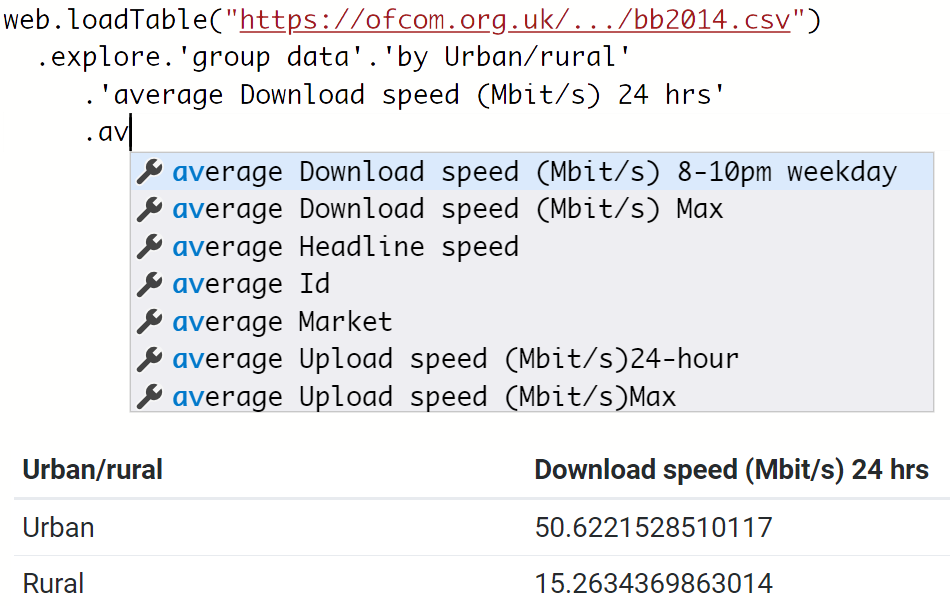
\includegraphics[scale=0.335]{gamma.png}
\caption{\small{TheGamma script that downloads and aggregates UK government data, running in 
  Wrattler notebook with a live preview.}}
\label{fig:gamma}
\vspace{-0.5em}
\end{figure}


%\begin{figure}
%\vspace{-0.5em}
%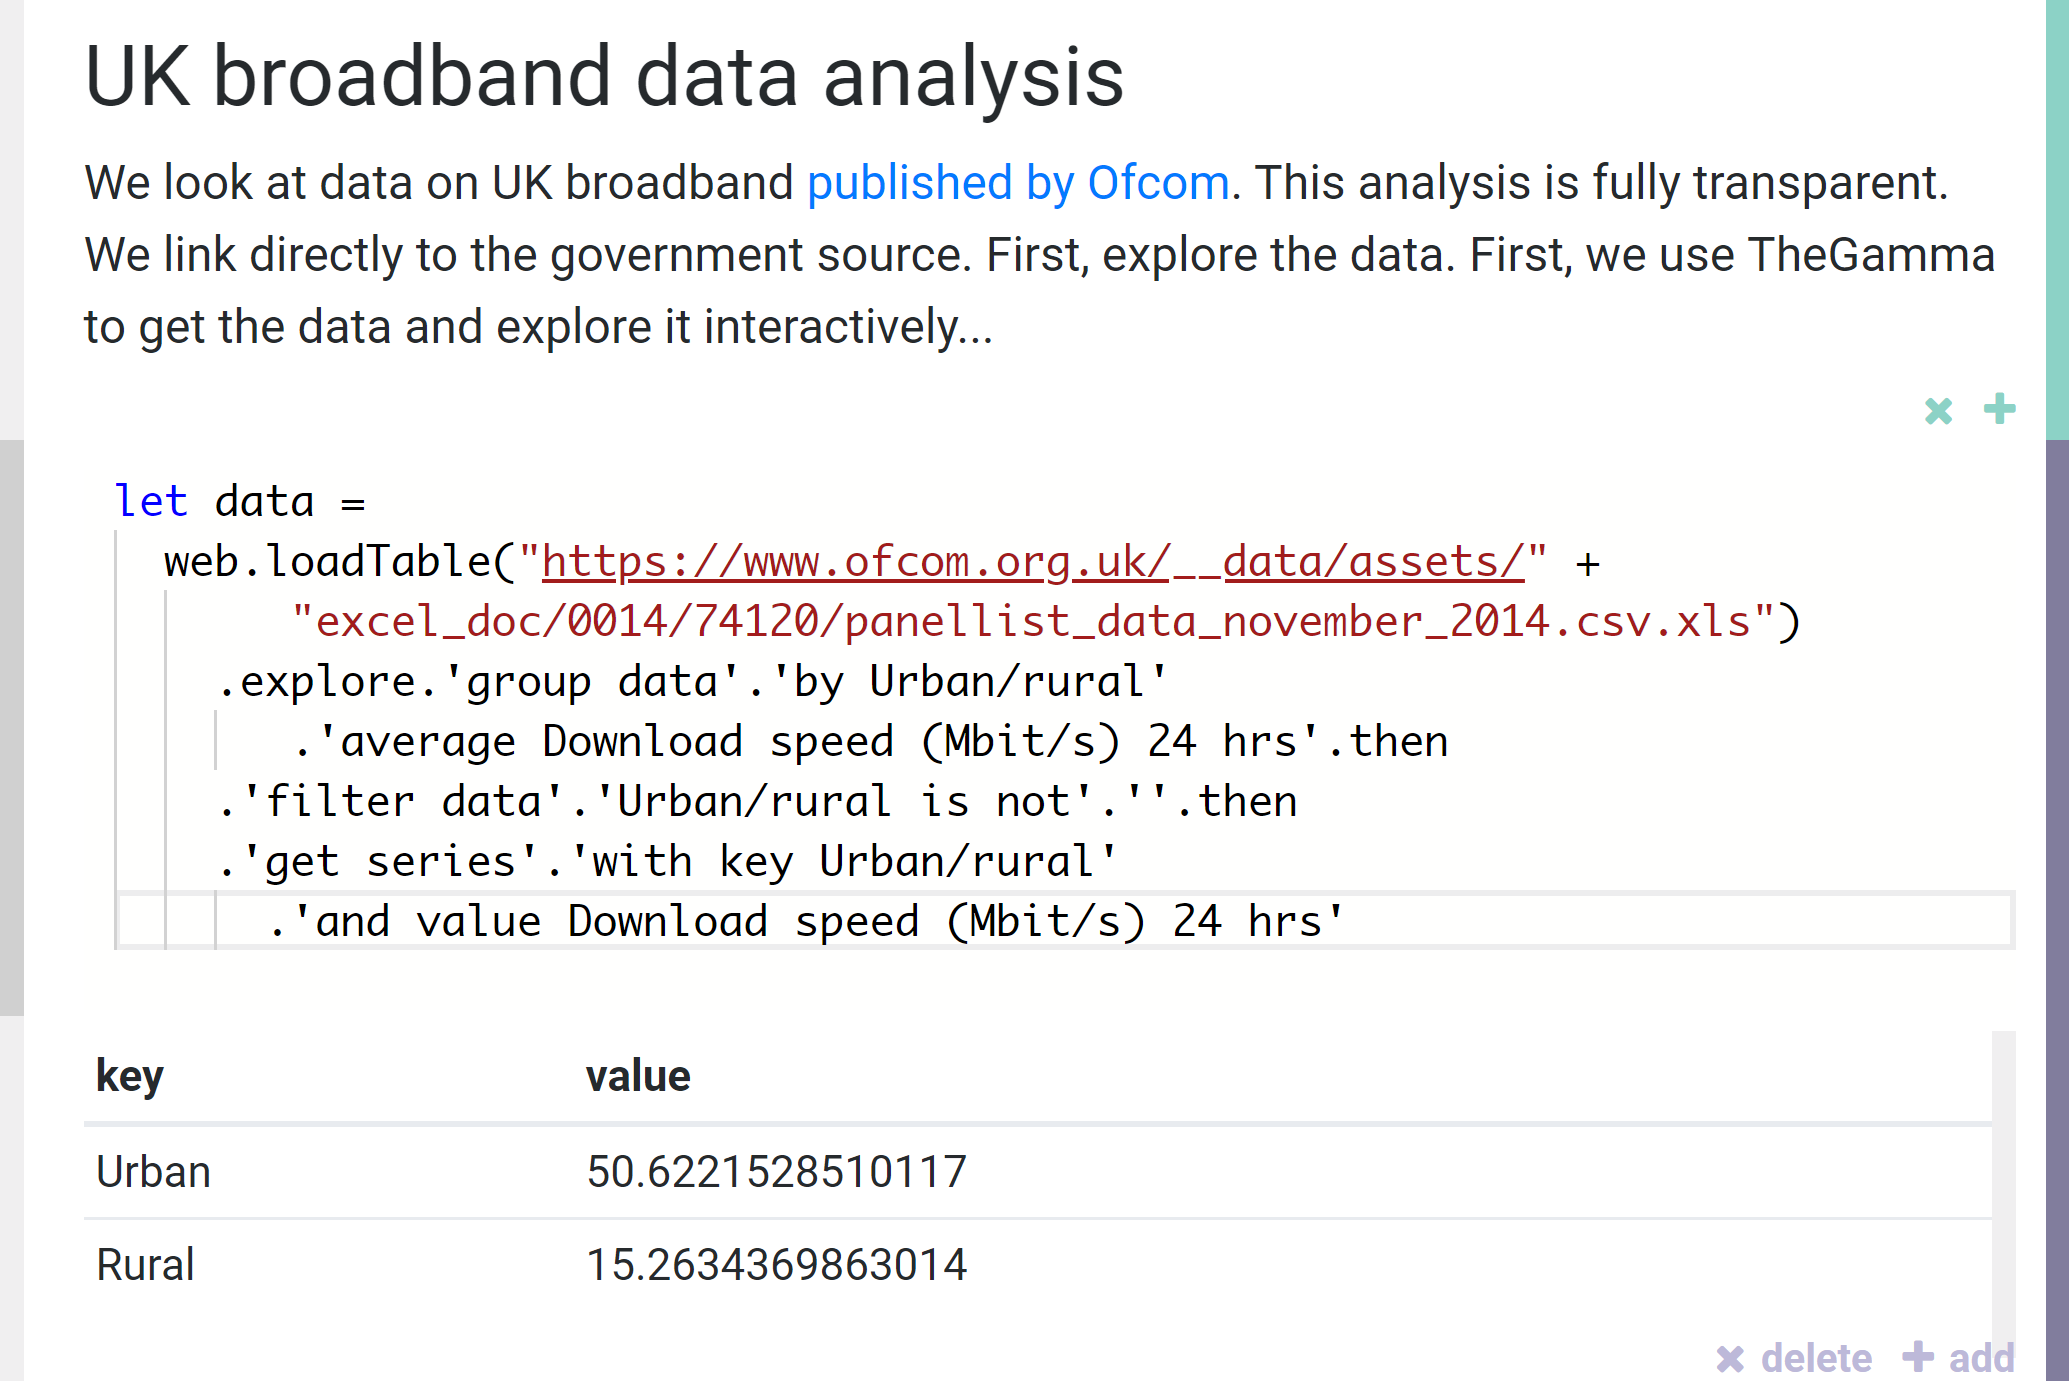
\includegraphics[scale=0.15]{screen.png}
%\caption{\small{TheGamma script that downloads and aggregates UK government data, running in 
%  Wrattler notebook with a live preview.}}
%\label{fig:proto}
%\vspace{-0.5em}
%\end{figure}

\section{Related work}

The work in this paper directly follows the work on IPython and Jupyter systems
\cite{ipython,jupyter}. Wrattler shares many properties with those and aims to address some
of their limitations. To address reproducibility, some Jupyter extensions and systems such
as R markdown %\cite{rmarkdown} 
lock cells after evaluation. 

Dataflow notebooks \cite{dataflow} attach unique hashes to cell 
evaluations. This allows the user to refer to dependencies explicitly and, in effect, construct
a dependecy graph manually.
Scientific workflow systems \cite{taverna,kepler} manage evaluation over a 
dependency graph similarly to Wrattler, but allow editing it directly via a GUI, rather
than through code in a notebook.

The noWorkflow project \cite{noworkflow} links the two approaches by instrumenting Jupyter 
kernel with a mechanism for capturing provenance based on light-weight annotations.
Vizer~\cite{vizer} focuses on integrating notebooks with spreadsheet-like interface.
It internally uses a data store component similar to ours, but does not keep dependency graph
on the client.

Our binding process is inspired by Roslyn~\cite{roslyn} and extends an
earlier work on TheGamma \cite{livegamma}. It is simiar to methods used in live programming 
languages \cite{live,subtext}, incremental compilation \cite{incremental} and
partial evaluation \cite{partial}. Wrattler adapts those methods to a notebook environment. 

\section{Summary}

This paper presents early work on Wrattler -- a new notebook system for data science that makes
notebooks reproducible, live and polyglot. The properties of Wrattler are enabled by provenance
information that is maintained thanks to two changes to the standard architecture of notebook 
systems. 

First, Wrattler separates the state management from code execution. This allows versioning,
polyglot notebooks and integration of third-party tools that can work directly with
the data store. Second, Wrattler keeps a dependency graph on the client (web browser) and uses 
it to control evaluation. This guarantees reproducibility and allows faster feedback during
development.

\begin{acks}
The authors would like to acknowledge the funding provided by the UK Government's Defence \& 
Security Programme in support of the Alan Turing Institute and the EPSRC grant EP/N510129/1.
We thank to our colleagues Chris Williams, Zoubin Ghahramani and Ian Horrocks and attendees 
of a recent AIDA project workshop.
\end{acks}

\bibliography{paper}
\end{document}
